\documentclass[12pt]{article}
\usepackage{longtable}
\usepackage{booktabs}
\usepackage{tabularx}
\usepackage{graphicx}
\usepackage{float}
\usepackage{fullpage}
\usepackage{longtable}
\usepackage{xltabular}
\usepackage{caption}
\usepackage{pdflscape}
\usepackage{afterpage}
\usepackage{multirow}
\usepackage[margin=1in]{geometry}
\usepackage{enumitem}
\usepackage{pdflscape}

\newcounter{assumpnum} %Assumption Number
\newcommand{\atheassumpnum}{P\theassumpnum}
\newcommand{\aref}[1]{A\ref{#1}}
\newcounter{haznum} %Hazard Category Number
\newcommand{\hthehaznum}{H\thehaznum}
\newcommand{\href}[1]{H\ref{#1}}
\newcounter{srnum} %SR Number
\newcommand{\srthesrnum}{SR\thesrnum}
\newcommand{\srref}[1]{SR\ref{#1}}
\newcounter{fmeanum} %Table Counter
\newcommand{\fmeathefmeanum}{\thefmeanum}
\newcommand{\fmearef}[1]{\fmearef{#1}}

\title{Hazard Analysis\\\progname}

\author{\authname}

\date{}

%% Comments

\usepackage{color}

\newif\ifcomments\commentstrue %displays comments
%\newif\ifcomments\commentsfalse %so that comments do not display

\ifcomments
\newcommand{\authornote}[3]{\textcolor{#1}{[#3 ---#2]}}
\newcommand{\todo}[1]{\textcolor{red}{[TODO: #1]}}
\else
\newcommand{\authornote}[3]{}
\newcommand{\todo}[1]{}
\fi

\newcommand{\wss}[1]{\authornote{blue}{SS}{#1}} 
\newcommand{\plt}[1]{\authornote{magenta}{TPLT}{#1}} %For explanation of the template
\newcommand{\an}[1]{\authornote{cyan}{Author}{#1}}

%% Common Parts

\newcommand{\progname}{Mechatronics Engineering} % PUT YOUR PROGRAM NAME HERE
\newcommand{\authname}{Team 10, LiDart
\\ Jonathan Casella
\\ Karim Elmokattaf
\\ Michaela Schnull
\\ Neeraj Ahluwalia} % AUTHOR NAMES                  

\usepackage{hyperref}
    \hypersetup{colorlinks=true, linkcolor=blue, citecolor=blue, filecolor=blue,
                urlcolor=blue, unicode=false}
    \urlstyle{same}
                                


\begin{document}
\pagenumbering{roman}

\maketitle

\newpage

\tableofcontents
\listoffigures
\listoftables

~\newpage

\section*{Revision History}

\begin{tabularx}{1.0\textwidth}{p{3cm}p{2cm}p{4cm}X}
\toprule {\bf Date} & {\bf Version} & {\bf Authors} & {\bf Notes}\\
\midrule
10\textbackslash Oct\textbackslash 2022 & 1.0 & Michaela Schnull \newline Kareem Elmokattaf  & Initial Release\\
\bottomrule
\end{tabularx}

~\newpage

\section{Reference Material}

This section records information for easy reference.

\subsection{Abbreviations and Acronyms}

\renewcommand{\arraystretch}{1.2}
\begin{tabular}{l l} 
  \toprule		
  \textbf{Symbol} & \textbf{Description}\\
  \midrule 
  A & Assumption\\
  ALARA & As Low as Reasonably Achievable\\
  FMEA & Failure Modes and Effects Analysis\\
  GUI & Graphical User Interface\\
  H & Hazard\\
  POST & Power-On Self-Test\\
  SR & System Requirement\\
  \bottomrule
\end{tabular}\\

\pagenumbering{arabic}

\section{Background}

3D scanning is a versatile technology that is used across many industries, but its uses are often limited by high cost
and complexity. \progname aims to build a low cost, simple to use 3D scanning robot. A software suite will process
data obtained from the robot and provide a user interface. \progname’s end product will be a wheel based mobile robot
with all required sensors on-board that can be connected to over WiFi.

\section{Introduction}

\subsection{Purpose}

The purpose of this document is to identify and provide actions to eliminate or mitigate hazards associated with the setup and operation of \progname. This document is intended to identify failure modes, effects, and causes related to system hazards. Recommended actions have been assigned to each failure mode and new requirements have been created to mitigate and eliminate hazards.

\subsection{Scope}
The \progname ~system consists of a graphical user interface that allows the user to remotely drive a robot, initiate 3D scans, and download the final stitched 3D scan. Hazard analysis will be performed on all processes relating to the installation and operation of the LiDart system.  Hazard analysis will not be completed for software components such as licensing, user authentication, security, and data storage as these considerations are not within the scope of the project. Failure modes due to human performance factors are not included in this hazard analysis.

\section{Assumptions and Definitions}

\subsection{Assumptions}

The following assumptions were used in the development of this process FMEA:

\noindent \begin{itemize}
\item[A\refstepcounter{assumpnum}\theassumpnum \label{Assumption1}:] The \progname ~system is in good condition. All maintenance activities have been properly completed. 

\item[A\refstepcounter{assumpnum}\theassumpnum \label{Assumption2}:]The \progname ~system has not been damaged or modified by the user.

\item[A\refstepcounter{assumpnum}\theassumpnum \label{Assumption3}:] The user will follow operating instructions as provided in the user manual.

\end{itemize}

\subsection{Definitions}

\subsubsection{Hazard}

The definition of a hazard used throughout this document is based on  Nancy Leveson's work. A hazard is defined as any property or condition of a system coupled with an environment that has the potential to cause harm, damage, or adverse effects.

\section{System Overview}

The \progname ~system is a 3D scanning solution in the form of a mobile robot. The system includes location markers, a remote-controlled robot, and a graphical user interface.

\subsection{System Boundary}

Hazard analysis is performed on \progname ~system, which consists of: 

\begin{itemize}
\item The physical robot, including the hardware and firmware running on the robot
\item Location markers
\item The GUI application
\item A WiFi network
\end{itemize}

The physical device running the GUI application and the environment surrounding the robot are not controlled by \progname. Hazard analysis will not be performed on elements external to the system.
 
\subsection{System Processes}

 \noindent The processes executed by the \progname ~system can be broken into the following categories:

\noindent \begin{itemize}
\item[\textbf{H\thehaznum \label{H0}}] \textbf{General Failure Modes}\\
Consists of the failure modes that may occur at any time. 

\item[\textbf{H\refstepcounter{haznum}\thehaznum \label{H1}}] \textbf{System Setup and Installation}\\
Before performing scanning operations, the robot must be powered on, and communication must be established between the robot and the user interface over WiFi. A series of functional checks are performed after communication is established to ensure the robot is in an operational state. Furthermore, location markers must be installed. Figure~\ref{fig_Setup} illustrates the setup and installation processes.
\begin{figure}[H]
\centering 
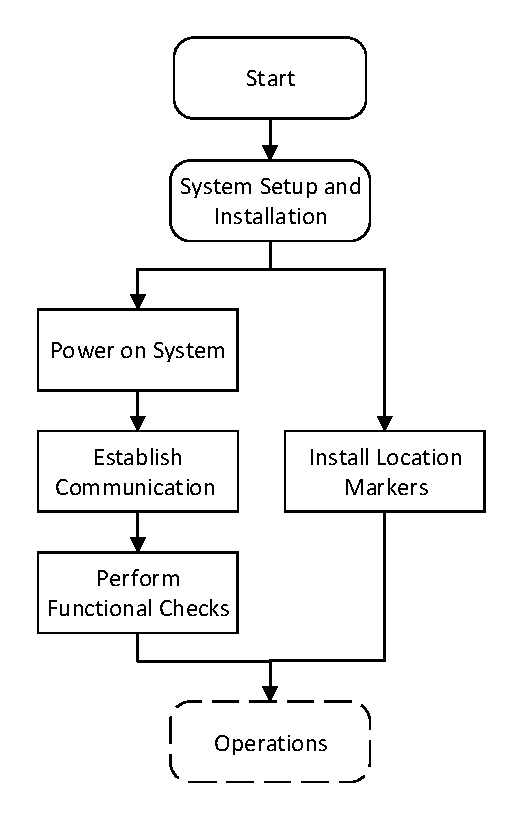
\includegraphics[width=0.5\textwidth]{Figures/Setup Processes.pdf}
\caption{Setup and Installation Process Diagram}
\label{fig_Setup}
\end{figure}

\item[\textbf{H\refstepcounter{haznum}\thehaznum \label{H2}}] \textbf{Operation}\\
While in operation, the robot must respond to inputs from the user and perform scanning operations. The system must perform state estimation, acquire sensor data, and output 3D models. Figure~\ref{fig_Operation} illustrates the operational process logic.
\begin{figure}[H]
\centering
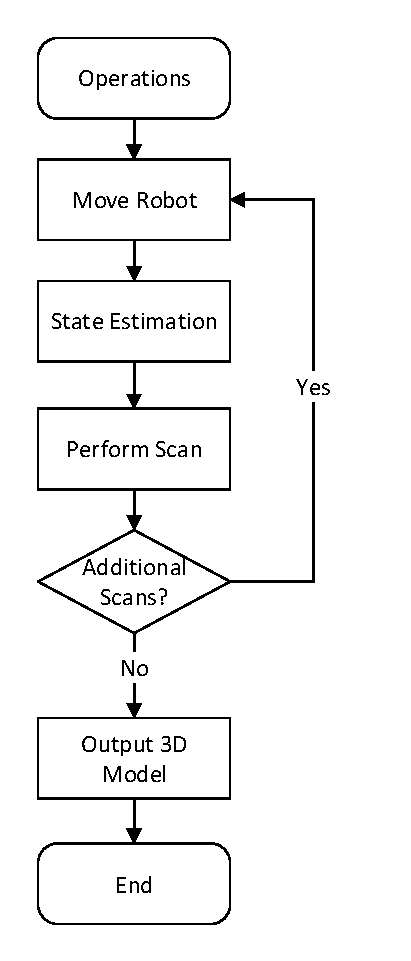
\includegraphics[width = 0.4\textwidth]{Figures/Operation Processes.pdf}
\caption{Operation Process Diagram}
\label{fig_Operation}
\end{figure}
\end{itemize}

\section{Failure Modes and Effects Analysis}

A Failure Modes and Effects Analysis (FMEA) is used to perform hazard analysis of the \progname ~system. The table is included in Appendix ~\ref{FMEA}.

\section{System Requirements}

New system requirements have been created based on failure modes identified in the FMEA. Existing system requirements that mitigate or eliminate hazards identified in the FMEA have been included for reference.

\subsection{New System Requirements}

\begin{itemize}

\item[\textbf{SR\refstepcounter{srnum}\thesrnum \label{SR1}}] The system shall prevent the robot from driving into an obstacle. An error message should be displayed if the user attempts to move the robot into an obstacle.
\newline Rationale: Driving into an obstacle could damage the robot and/or the surrounding system. The system should prevent the user from driving the robot into an obstacle and have a means of notifying the user about the obstacle.

\item[\textbf{SR\refstepcounter{srnum}\thesrnum \label{SR2}}] The system shall prevent the robot from moving during scanning operations.
\newline Rationale: The data acquired by the sensor may not be correct if the robot is moving during data acquisition.

\item[\textbf{SR\refstepcounter{srnum}\thesrnum \label{SR3}}] The system shall automatically save data from scanning operations.
\newline Rationale: Data should be saved automatically  without requiring the user to manually save it in case of unexpected events that cause data loss.

\item[\textbf{SR\refstepcounter{srnum}\thesrnum \label{SR5}}] The system shall validate all user inputs on the GUI.
\newline Rationale: Incorrect inputs may cause unexpected system behaviour.

\item[\textbf{SR\refstepcounter{srnum}\thesrnum \label{SR6}}] The robot's electrical system shall use short circuit protection devices.
\newline Rationale: Short circuit protection should be implemented as a safety precaution and to protect electrical devices.

\item[\textbf{SR\refstepcounter{srnum}\thesrnum \label{SR7}}] An adequate number of location markers shall be used such that the robot can determine it's location in any position.
\newline Rationale: The system must be able to perform localization in any position in order to stitch point cloud data.

\item[\textbf{SR\refstepcounter{srnum}\thesrnum \label{SR8}}] The robot shall perform a power-on self-test (POST) to check the functionality of system components prior to operation.
\newline Rationale: The POST will identify functional issues and mitigate downstream functional and performance issues.

\item[\textbf{SR\refstepcounter{srnum}\thesrnum \label{SR10}}] The system shall display a warning if there is insufficient data acquired to create a 3D model.
\newline Rationale: The point stitching algorithm requires sufficient data to create a 3D model. The accuracy of the model may decrease or a model may not be able to be created if there is insufficient data.

\item[\textbf{SR\refstepcounter{srnum}\thesrnum \label{SR11}}] The system shall be able to retroactively correct stitched point cloud models given new data.
\newline Rationale: If there is an issue with a certain section of a 3D model, the system should be able to correct the model given new data for that section. The user should not have to re-scan every section.

\end{itemize}

\subsection{Existing System Requirements}

\begin{itemize}

\item[\textbf{SR\refstepcounter{srnum}\thesrnum \label{SR4}}] The robot shall be placed in a safe-state if communication with the GUI is lost.
\newline Rationale: The robot must not be able to move if communication with the user is lost.

\item[\textbf{SR\refstepcounter{srnum}\thesrnum \label{SR9}}]All hardware and electronic components shall be easily accessible.
\newline Rationale: Electrical components should be easily accessible for trouble-shooting and maintenance purposes.

\end{itemize}

\section{Roadmap}

New system requirements created from the hazard analysis will be implemented throughout the design phase of this project to eliminate and mitigate hazards. The principle of ALARA will be used to reduce risk and decide which requirements will be implemented. 


\afterpage{
\newgeometry{margin=0.5in}
\begin{landscape}
\centering
\appendix
\section{Failure Modes and Effects Analysis}
\label{FMEA}
\tiny
\captionof{table}{Failure Modes and Effects Analysis}
\begin{xltabular}{\linewidth}{|p{3cm}|p{1cm}|p{3.25cm}|p{3.25cm}|p{3cm}|p{3cm}|p{4cm}|X|}
\hline
\textbf{Design Component} & \textbf{Ref.} & \textbf{Failure Mode} & \textbf{Cause of Failure} & \textbf{Effect of Failure} & \textbf{Detection} & \textbf{Recommended Actions} & \textbf{SR}\\
\hline
\multicolumn{8}{|c|}{\textbf{General Failure Modes}}\\

\hline
GUI & H0-1 & GUI crashes & 1. Poor software memory management and performance \newline 2. Unexpected error handling & 1. Communication with the robot is lost \newline 2. The robot continues to move after communication is lost \newline 3. Current scanning data is lost & The GUI closes unexpectedly & 1. Validate all user inputs to the GUI \newline 2. Place the robot in safe-state if communication is lost \newline 3. Provide an auto-save feature to ensure data is not lost & \srref{SR5}\\

\hline
\multirow{2}{*}{System Power} & H0-2 & Power is lost & 1. Battery died \newline 2. Cables/wires become disconnected & 1. The robot no longer functions and may be completely halted & The system will not power-on or powers down & 1. Charge or replace the battery \newline 2. Connect any disconnected cables/wires & \srref{SR9}\\\cline{2-8}
& H0-3 & Short circuit & 1. Loose electrical connections \newline 2. Damaged electrical components \newline 3. Buildup or surges of electricity & 1.Electrical components may be damaged \newline 2. The robot stops working & Sparking and power system issues & 1. Power off the robot and investigate the cause of the short circuit \newline 2. Replace damaged components \newline 3. Use circuit protection devices & \srref{SR6}, \srref{SR9}\\

\hline
\multicolumn{8}{|c|}{\textbf{System Setup and Installation}}\\

%Establish Communication
\hline
Establish Communication & H1-1 & Cannot establish communication with the robot & 1. Incorrect network settings \newline 2. Robot is not in the range of the network \newline 3. Hardware/system power failure & 1. Delay to investigate and fix network issues & Error message on the GUI when attempting to connect to a network & 1. Move the robot to a location with a strong network signal \newline 2. Check the network settings, and correct the settings if necessary \newline 3. Reset the network \newline 4. Power cycle the robot & \srref{SR9} \\

%Functional Checks

\hline
Functional Checks & H1-2 & Functional checks (e.g. check that all required devices are connected, sensors are calibrated) are not successful & 1. Checks fail when they should pass & 1. Delay to investigate and fix any errors & An error message on the GUI stating which checks failed & 1. Display a warning on the GUI stating which checks failed \newline 2. Investigate and fix system components that have failed & \srref{SR8}, \srref{SR9}\\

\hline
\multicolumn{8}{|c|}{\textbf{Operation}}\\

%Communication
\hline
Communication & H2-1 & Communication between the GUI and the robot is lost & 1. The WiFi signal is too weak \newline 2. The WiFi signal intermittently cuts out & 1. The robot will not be able to be controlled by user \newline 2. Data loss & Error messages on the GUI that the robot cannot connect to a network & 1. Keep the robot within the range of the WiFi signal & \srref{SR3}, \srref{SR4}\\

%Movement of robot
\hline
\multirow{2}{*}{Movement of Robot} & H2-2 & The robot crashes & 1. The robot does not respond to user input \newline 2. The robot is not capable of stopping in time & 1. Damage to the surrounding environment \newline 2. Damage to the robot & Visual inspection & 1. Display a warning on the GUI when the robot is getting too close to an obstacle \newline 2. Use software controls to prevent user input from instructing the robot to drive into an obstacle & \srref{SR1}\\\cline{2-8}

%State Estimation
\hline
\multirow{2}{*}{State Estimation}  & H2-3 & The location of the robot cannot be determined & 1. The location markers are not in the camera(s)' field of view \newline 2. The object detection algorithms cannot identify the location markers \newline 3. Inadequate number of location markers & 1. The system cannot stitch point cloud data and create a 3D model &  The GUI displays a message that the state cannot be estimated & 1. Re-calibrate the system \newline 2. Ensure enough markers are used \newline 3. Adjust the position of the location markers so that they are visible to the robot \newline 4. Move the robot to a new location & \srref{SR7}\\\cline{2-8}
& H2-4 & False positive that the state is correctly estimated & 1. State estimation filtering error & 1. The 3D model output is incorrect & Visual inspection of 3D model output & 1. Automatically save data so that the scans performed prior to incorrect localization are not lost \newline 2. Re-scan the affected area & \srref{SR3}, \srref{SR11} \\\cline{2-8}

%Perform Scan
\hline
\multirow{2}{*}{Perform Scan} & H2-5 & Insufficient amount of data acquired & 1. Not enough scans are performed & 1. A 3D model cannot be created \newline 2. The accuracy of the 3D model may decrease & An error message on the GUI stating not enough scans when the system attempts to process data & 1. Perform additional scans & \srref{SR10}\\\cline{2-8}
& H2-7 & The data acquired is not correct & 1. Sensor malfunction \newline 2. The robot moves during data acquisition & 1. 3D models are inaccurate & Visual inspection of 3D model output & 1. Use software controls to prevent the robot from moving during scanning & \srref{SR2}\\\cline{2-8}
\hline

\end{xltabular}
\end{landscape}
\clearpage% Flush page
}

\end{document}